% !TEX root = ../Dissertation.tex
% !TEX spellcheck = en_US

% THIS IS THE SECOND CHAPTER %
\noindent 
This chapter explains the survivable algorithms and their sharp differences in their blocking, failure and resource allocation by introducing failures described in the chapter 4.

\section {Effects of Failure Assumptions}

All these values discussed in the previous sections, have various impact on failures analysis. Some of them are discussed in this section.
\begin{enumerate} [leftmargin=*]
\item The simulation is set to run for a 1 year period (8760 hours) and total failures in this duration happens to be 63. This is due to the constant number of failures in every sub-interval.

%Table 4.3 Periodic failure counts
\begin{table}[!htbp]
\centering
\caption{Periodic failure counts}
 	\begin{tabular}{|c|c|}
	\hline\hline
	\textbf{Period(in hours)} & \textbf{Number of failures}\\
	\hline
	0 - 10000&72\\
	10000-20000&63\\
	20000-30000&56\\
	30000-40000&69\\
	\hline
	\end{tabular}
\end{table}

\item The time between the arrival of each failure is also constant over a period of 100000 hours. Because of this reason, the simulation time is set to 1 year as the trend is expected to replicate after this period. Figure 4.3 attempts to prove the memoryless property of Poisson.
%Fig. 4.3 Time between failures

\begin{figure}[hbt!]
\centering
\includegraphics[page=34, width=12cm, height=8cm]{fig18.png}
\caption{Failure arrivals over time}
\label{fig:failureArrivals}
\end{figure}

\item Overlaps are very rare yet some accidental overlaps tend to happen due to more number of long distance links. It is normal to observe this trend due to presence of number of overseas links and it's higher MTTR.
%Fig. 4.4 Link failure Overlaps
\begin{figure}[hbt!]
\centering
\includegraphics[page=34, width=12cm, height=8cm]{fig19.png}
\caption{Link failure overlaps over time}
\label{fig:failOverlaps}
\end{figure}

\end{enumerate}

\indent It can be observed that majority of simulation time has no or one failures. Rarely, the overlaps happen and the intensity fades away for three and four overlaps. This is illustrated in figure 4.4. This scenario is good for survivability analysis as connection would still be able to survive in the event of single link failures in the system.

\section {Setting up the environment}

\section {Factors Inducing Failure of a Connection}
This section describes how these failure assumptions impact connection failures in ESnet. These impacts may be the result of network design and have a varying impact from one network to other. Probing in to such details will set it up and makes it easy to examine the results in the upcoming chapters.

\subsection {MTBF and MTTR}
The MTBF and MTTF are parameters of failure and they directly impact connection failures. To obtain these results, Unicast connection traffic has been generated for the stipulated simulation time.
			
%Table 4.5 Effect of blocking w.r.t MTTF
\begin{table}[!htbp]
\centering
\caption{Failure Effects of variation FITs}
 	\begin{tabular}{|c|c|c|}
	\hline\hline
	\textbf{FIT/km} & \textbf{Load} & \textbf{Failure Probability}\\
	\hline
	114&100&0.03\\
	314&100&0.13\\
	\hline
	\end{tabular}
\end{table}

From the table 4.4, the increase in the failure is directly proportional to the increase FIT. This is due to unavailability of links for longer periods. Also, the values 

Usually failure rates can be 114 FIT/km, 184 FIT/km and 314 FIT/km. This research considers 114 FIT/km as backbone networks are assumed to be most reliable.

\subsection {Distance and hop counts}
One underlying assumption in this section is that greater hop counts is directly proportional to the longer path. This is valid as pretty much all networks are built this way. Longer paths can sometimes be an indication of network in high blocking state and it is about to reach steady state. Further increase in load may not be a good idea as graph is divided into small number of sub-graphs which may result in less number of hop counts and this is different from the shorter paths at lower loads. This is one of the many reasons in this research why the network was not tried for higher values of load.

%Fig. 4.6 Effect of Hop counts
\begin{figure}[hbt!]
\centering
\includegraphics[page=34, width=12cm, height=8cm]{fig20.png}
\caption{Effect of distance w.r.t failure}
\label{fig:distanceFailure}
\end{figure}


\indent Connections set up with longer paths are also prone to link failures. Because longer paths cover more number of long distance links to get to the destination thus the probability that one of the links getting failed will also increase. This will also get us in to thinking that connections set up in the network which is in high blocking state would result in more number of failures.

\indent It is evident from [1] that anycast has spatial advantage over unicast but also indirectly effects failures. The anycast in OSCARS 1.0 prototype is built in such a way that a path with minimum cost is preferred over others [1].  The idea here is to decrease the resource allocation which may assist in decrease in failures as well.
	
\section {Holding time}
Like hop count, increase in holding time of the connection increases the probability of connection getting failed. Because the longer the connection stays, greater the chance of link failures. 
%Fig. 4.7 Effect of holding time

\begin{figure}[hbt!]
\centering
\includegraphics[page=34, width=12cm, height=8cm]{fig21.png}
\caption{Holding time Vs Failure}
\label{fig:holdFail}
\end{figure}


\indent All these values MTTR, holding time are tuned up in such a way that network could be operated for lower blocking and failure.
	
%Fig.5.1 Setting up the Environment
\begin{figure}[hbt!]
\centering
\includegraphics[width=15cm, height=10cm, page=18]{fig22.png}
\caption{Setting up the environment}
\label{fig:setEnv}
\end{figure}

	As discussed in the previous chapters, the traffic generator is merely a client connects to the controller OSCARS and generates traffic making use of API. For every request, 
OSCARS calculate path and responds with the format specified in the chapter 2. Note that these requests are submitted to OSCARS one at a time. 

\section {Effects of Palindromic Path}

	In commercial networks, the forward and reverse path for a {($S->D$)} does not necessarily have to be the same. In other words, they are mostly non-palindrome (Forward and reverse path are not same). But in a private domain sometimes, palindrome may be strictly preferred over non-palindrome. For instance, OSCARS gives priority to palindrome but also keeps the option of non-palindrome open on demand. This demand may impact failure and blocking. It is presumed that non-palindrome brings more links in to equation to set up a connection and therefore, increases the probability of failure of connection. That said, it is also possible to have reduced blocking in case of non-palindrome because this does not enforce a connection to be palindrome. Figure 5.2 illustrates the working of this PCE in OSCARS.


%Fig. 5.2 Effects of Palindrome
\begin{figure}[hbt!]
\centering
\includegraphics[width=15cm, height=10cm, page=18]{fig23.png}
\caption{Palindromic PCE in ESnet}
\label{fig:palinPCE}
\end{figure}

\subsection {Palindrome}
	For the sake of this example, the bandwidths mentioned in the above topology are assumed to be available in one direction. Let's say if a user requests bandwidth 20 Gbps from A to E, controller fails to find the path with the palindrome option. Both the paths AFE and ACDE can only allocate resources for forward path because the maximum available bandwidth is 20 Gbps. In this research, this can be considered as a block as it fails to allocate resources for the connection. 

\subsection {Non-Palindrome}
	Non-palindrome being an option, controller would be able to identify that for the given pruned network, it is not possible to set a palindromic connection. But it does not give up there. This time it calculates if there could be any other reverse paths available. In the above topology, controller would be able to set up the connection with AFE as forward and EDCA for reverse path. This is a successful set up of a connection.  

\section {Performance Analysis}

%Fig. 5.3 Palindrome Vs Non-Palindrome Blocking

\begin{figure}[hbt!]
\centering
\includegraphics[width=12cm, height=8cm, page=18]{fig24.png}
\caption{Palindrome Vs Non-Palindrome - Blocking}
\label{fig:palinBlock}
\end{figure}

Blocking probability is the ratio of number of blocked connections  to the total number of connections.

%Fig. 5.4 Palindrome Vs Non-Palindrome Failure

\begin{figure}[H]
\centering
\includegraphics[width=12cm, height=8cm, page=18]{fig25.png}
\caption{Palindrome Vs Non-Palindrome - Failure}
\label{fig:palinBlock}
\end{figure}

Failure probability is the ratio of number of failed connections to total number of successful connections.

Above results seems to suggest that Non-palindrome did not have any advantage in terms of blocking probability if the forward and reverse bandwidths for connection are same (not shown here). This trend seems to continue for asymmetric bandwidth requests as well.  The trend lines of palindrome and non-palindrome overlap during the entire period. In fact, non-palindrome performs worse for some of the load values. Because the return paths of some of the connections tend to take a longer route, thus contributing to the blocking of new logical connections. Failure plots further strengthen palindrome because non-palindrome seems to fail little more often. This is due to the reason briefly explained in the chapter 4.5.

The data above helps in directing the future analysis of survivability to fix on palindrome. Therefore, the simulation is run for specifications, Palindrome and Symmetric Bandwidth.

\section {Comparative analysis of unicast survivability}

This section discusses how the survivability algorithms, Iterative SP and Bhandari perform and tries to explore the effective resource allocation of these two survivable algorithms.

\subsection {Blocking Probability}

%Fig. 5.5 Iterative SP Vs Bhandari Blocking

\begin{figure}[H]
\centering
\includegraphics[width=10cm, height=8cm, page=18]{fig26.png}
\caption{Iterative disjoint SP Vs Bhandari - Blocking}
\label{fig:iterVsBhBlock}
\end{figure}

This behavior is already discussed in the chapter 2.3.2. Iterative Djikstra is greedy in allocating resources and therefore, it may lead to more blocking than Bhandari. This chart confirms that in this network, iterative SP has effected roughly up to 2\% increase in blocking probability at higher loads. 

\subsection{Resource allocation}

%Fig. 5.6 Resource allocation
	
\begin{figure}[H]
\centering
\includegraphics[width=10cm, height=08cm, page=18]{fig27.png}
\caption{Iterative SP Vs Bhandari - Hop counts}
\label{fig:iterVsBhHops}
\end{figure}
	
The Number of hops is the average number of hops for all successful connections from a source to destination in one direction.
	
Figure 5.6 shows that average hop counts decreases by 1 for both primary and backup paths of iterative Djikstra. This shows that the logical connections set up with Bhandari may be slower and using more resources than iterative Djikstra even at lower loads with almost zero blocking. But decreased hop counts may positively approach failures. Let's see if this assumption is true in the following section.

\subsection{ Failure Probability }
%Fig. 5.7 Failure Probability

\begin{figure}[hbt!]
\centering
\includegraphics[width=10cm, height=8cm, page=18]{fig28.png}
\caption{Iterative disjoint SP Vs Bhandari - Failure}
\label{fig:iterVsBhFailure}
\end{figure}

Surprisingly, the reduced hops of iterative Djikstra does not provide any advantage over Bhandari for failure. Shorter paths are expected to experience less number of failures. Iterative Djikstra, although takes less number of hops to reach the destination, it still should travel the same distance as Bhandari. Due to this, paths of iterative Djikstra may use more number of long distance links as a result of reduced hop counts. Remember, the decrease in the anycast failure is because the destinations are different and controller OSCARS may choose the destination with shortest path based on cost. But in survivability, there is only one destination and its distance from source for primary paths in both the approaches are almost same.

Fig. 5.8 explains the case where the iterative Djikstra is forced to use a link of distance 2018 km whereas Bhandari could reach with medium or short distance links. Remember, the failure of the each link is independent and directly proportional to distance. Hence, in the below example, both the paths have equal chance of failure. 

%Fig. 5.8 Path Illustration
\begin{figure}[H]
\centering
\includegraphics[width=15cm, height=10cm, page=18]{fig29.png}
\caption{Illustration of path distance for primary and backup paths}
\label{fig:ipathIllustration}
\end{figure}

To explore more on this, the failure probability is calculated for individual paths to see if that is true. It appears that backups have failed more than primary but between primary or backup, there is not much difference. This proves that backup paths are actually taking the longer route in terms of costs, hops and distance for both iterative approach and Bhandari.

%Fig. 5.9 Path Failures
\begin{figure}[H]
\centering
\includegraphics[width=12cm, height=8cm, page=18]{missing.png}
\caption{Individual path failures of Iterative and Bhandari}
\label{fig:ipathIllustration}
\end{figure}

Although resources impact network, blocking is given preference as connections need to be committed. Besides, failures also did not seem to favor iterative Djikstra. Further, resource allocation of Bhandari is still optimal at higher load. Because of these reasons, Bhandari seems to be a convenient option for protection. But, this is not the end of the story for iterative Djikstra because the blocking probability of both the survivable approach at very low load does not seem to differ much. Can we exploit this behavior? Read on to know more about this in the next chapter.











